%%This is a very basic article template.
%%There is just one section and two subsections.
%\documentclass[12pt,oneside,a4paper,doublespacing]{article} % for submission
\documentclass[11pt,oneside]{article} % for sharing


\usepackage{appendix}
\usepackage{amsmath}
\usepackage{array}
\usepackage{caption}
\usepackage{placeins}
\usepackage{graphicx}
\usepackage{subcaption}
\usepackage{longtable}
\usepackage{setspace}
%\usepackage{tikz}
\usepackage{booktabs}
\usepackage{xcolor,colortbl}
\usepackage{chngpage}
%\usepackage[active,tightpage]{preview}
\usepackage{natbib}
\bibpunct{(}{)}{,}{a}{}{;} 
\usepackage{url}
\usepackage{nth}
\usepackage{authblk}
%\usepackage{pdfsync}

\renewcommand{\listtablename}{List of Appendix Tables}
\newcolumntype{C}[1]{>{\centering\let\newline\\\arraybackslash\hspace{0pt}}m{#1}}
\newcolumntype{L}[1]{>{\raggedright\let\newline\\\arraybackslash\hspace{0pt}}m{#1}}
%\newcolumntype{C}{ >{\centering\arraybackslash} m{4cm} }
% working on this need to concatenate file name based on sex and variable name
%\newcommand\Cell[1]{{\raisebox{-0.05in}{\includegraphics[height=.2in,width=.2in]{Figures/ColorCodes/\expandafter#1}}}}  

\newcommand\ackn[1]{%
  \begingroup
  \renewcommand\thefootnote{}\footnote{#1}%
  \addtocounter{footnote}{-1}%
  \endgroup
}
\newcommand{\hm}[2]{\includegraphics[scale=.31]{Figures/HeatTables/1915/#1#2.pdf}}
\defcitealias{HMD}{HMD 2015}

% end preamble
%-------------------------------------------

\begin{document}

\title{Time-to-death patterns in markers of age and dependency}

\author[1]{Tim Riffe\thanks{riffe@demogr.mpg.de}}
\author[2]{Pil H. Chung}
\author[3]{Jeroen Spijker}
\author[4]{John MacInnes}
\affil[1]{Max Planck Institute for Demographic Research}
\affil[2]{Department of Demography, University of California, Berkeley}
\affil[3]{Centre d'Estudis Demogr{\`a}fics}
\affil[4]{School of Social and Political Science, University of Edinburgh}

%\author{[Authors]}


\maketitle

\begin{abstract}
We aim to determine the extent to which variables commonly
used to describe health, wellbeing, and disability in old-age vary primarily
as a function of years lived (chronological age), years left (thanatological
age), or as a function of both.
We analyze data from the US Health and Retirement Study to estimate chronological age and time-to-death patterns in 78 such variables. We describe
results from the birth cohort born 1915-1919 in the final 12 years of life. Our results show
that most markers used to study well-being in old-age vary along both the age
and time-to-death dimensions, but some markers are exclusively a function of
either time to death or chronological age, and others display different patterns
between the sexes.\ackn{We would like to thank the editors of this issue, who also organized the 2014 conference that inspired us to undertake this project. We also thank two anonymous reviewers whose comments improved the manuscript greatly. Research reported in this manuscript
was supported by the U.S. 
National Institute On Aging of the National Institutes of Health under award
numbers R01-AG011552 and R01-AG040245, the Spanish Ministry of Economy and
Competitiveness under award RYC-2013-14851, and the UK ESRC grant ES/K004611/1. The content is solely the
responsibility of the authors and does not necessarily represent the official views of the funding agencies.}
\end{abstract}

\section*{Background}

For an
individual, age across the life course consists of two components: time since
birth and time to death, the \textit{chronological} and \textit{thanatalogical}
dimensions of age, respectively. In the aggregate, thanatological age is determined
by the mortality rate schedule to which a birth cohort is subject until its
extinction. Individuals do not know their thanatological age with certainty. To
guess this quantity one projects an expectation of lifespan\footnote{Lifespan
is used throughout as a synonym for chronological age at death, or
thanatological age at birth. These concepts are identical with length of life,
which is not to be confused with life expectancy, the mean length of life..}
based on scenarios or extrapolations of how mortality rates might change over time. Data classified by chronological age, like census population counts, can be reclassified into thanatological age in this way \citep{brouard1986structure}.

Prospectively, decreasing mortality is equivalent to moving population into
higher thanatological ages, thereby increasing remaining life expectancy \citep{sanderson2005average}. In this case,
the notion and measure of future remaining lifespan is elastic, subject to
uncertainty.
In retrospect (after the death of a cohort), the thanatological age structure of
a cohort at a given past point in time is a fixed characteristic. Since a closed
birth cohort is akin to a stationary population,\footnote{The age structure of a birth cohort over time is proportional to the survivorship column of its lifetable, which is proportional to the stable age structure determined by the Lotka-Euler renewal model when the intrinsic growth rate is equal to zero.} one may be
tempted to assume that since chronological and thanatological age structures are
symmetrical in stationary populations
\citep{brouard1989mouvements,vaupel2009life,pancho2015} that the patterns of
demographic characteristics within cohorts might also demonstrate an
analogous kind of symmetry.
This is not so; even in the case of stationary populations or extinct cohorts,
the age profiles of other demographic characteristics in the population are decidedly different when
viewed chronologically versus thanatologically. If the demographic
characteristics in question are states, such as health states, one can confirm
that for cohorts the mean duration spent in each state is indeed identical, no
matter whether measured by chronological or thanatological age. Cohort
expectancies are immune from age classification biases. However, distinct
patterns emerge in period aggregates due to an interaction between lifespan
variation and the age profiles of demographic characteristics. 

Some life
transitions, states, and changes in state intensities are almost exclusively a
function of time to death. When we state that a characteristic is a
function of either age perspective we do not imply that age causes the given characteristic to vary, but rather that a characteristic varies in some smooth, regular, or parsimonious way over age. There are other instances where chronological age captures almost all pertinent variation. In cases where a characteristic strongly varies as a
function of time to death,
the common practice of aggregation over chronological age may misrepresent time
trends and misguide analyses about change over time and expectations for the
future. Measurement of the
end-of-life trajectories of characteristics is useful in such cases as a way of separating
mortality patterns from patterns in characteristics themselves.
Characteristic measurements are taken while the respondent is alive, but
thanatological age at each observation is unknown until the date of death is
known, and it is therefore retrospectively assigned. This final analytical step
lends clarity to the understanding of how characteristics vary within and
between lifespans.

Incorporating a time-to-death perspective in demographic studies is especially
important when assessing the impact of ``population aging.''
To the extent that the health, welfare, and social care demands of a
population are functions of thanatological rather than chronological age
structure, forecasts of the social and economic ``costs'' of aging that are
based only on chronological age profiles are prone to bias
\citep{stearns2004time}.

Research exploring time-to-death patterns has been done in other
domains, and topics examined can be roughly categorized into two types: 1)
things that are a function of apparent or perceived time to death
\citep{hamermesh1985expectations,hurd1995evaluation,carstensen2006influence,gan2004subjective,biro2010subjective,salm2010subjective,van2010living,cocco2012longevity,payne2013life,balia2013survival},
and 2) things that are a function of actual time to death
\citep{miller2001increasing,seshamani2004longitudinal,werblow2007population,
wolf2015disability,stearns2004time}.
The first kind are mostly studies on cognitive transitions and economic or
health behaviors, while the second kind are mostly studies on health
expenditure, except \citet{wolf2015disability}, which proposes a model to
separate latent time-to-death trajectories.
A third branch of research relates perceived and actual remaining lifetime
\citep{perozek2008using,delavande2011differential,post2012longevity,kutlu2013individuals}.
In this paper we will expand the second group, focusing on a broad range of
questions from ten waves of the US Health and Retirement Study \citep{HRS}.

We aim to understand the end-of-life age patterns of various dimensions of
morbidity, as measured by a set of 78 characteristics and indices. To do this,
we score the degree to which these characteristics vary in terms of thanatological
age, chronological age, or both. In all, we define four different age and
lifespan pattern families, which we use to classify the end-of-life prevalence
of each characteristic tested. The pattern of variation exhibited by a given
characteristic ought to determine how we measure, understand, and respond to the
characteristic. We show that often chronological age ought to be used in conjunction with thanatological age in order to classify patterns, but in many cases
chronological age provides no information at all, and it even obfuscates true temporal
patterns.

Our analytical approach is retrospective rather than
prospective, meaning that no lifetable assumptions are made in the measurement
of thanatological age, and no censoring adjustments are necessary. Although more
data are available for earlier and later cohorts, we report results only for the
cohort born from 1915 to 1919, which contains the most extensive set of observations in
the dataset used. In the following section we describe the methods in
greater detail. We then demonstrate the four primary age patterns by way of
example, and summarize all characteristics tested in terms of these four
patterns.
Finally, we discuss some implications and applications of this work.


\section*{Data \& Method}

All findings reported in this paper are based on data from the US Health and
Retirement Study (HRS). We use version M of the RAND edition of the data, which
is conveniently merged across all ten waves available as of 2013.
These data are free to download, and all details of data processing and methods are made freely available in an open code
repository.\footnote{This
repository includes R code used to process data, as well as generate results and
figures: \url{https://github.com/timriffe/ThanoEmpirical}}

We restrict the sample to only those
individuals born between 1900 and 1930 who died between 1992 and 2011, which
narrows the dataset down to 37,051 interviews of 9,238 individuals. Of
these interviews, 8,137 are from the 1,919 individuals who died from the
1915-1919 cohort. Observations from earlier and later cohorts are kept for the
sake of adding information when fitting models to the data.
%
\begin{figure}[!h]
\centering
\caption{Chronological age and thanatological age over the lifecourse of a birth
cohort}
\label{fig:LexisOrtho}
	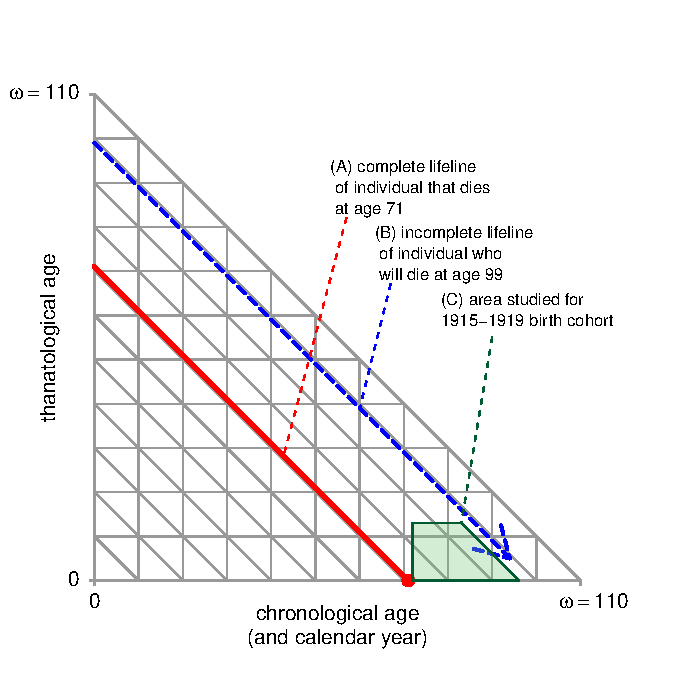
\includegraphics{Figures/Figure1.pdf}
\end{figure}

Underpinning this investigation are a series of demographic surfaces indicating
the average prevalence of a given marker along chronological and
thanatological time axes within a series of quinquennial birth cohorts, from
which we focus only on the central 1915-1919 birth cohort.
This visual tool is similar to but orthogonal to the familiar Lexis surface.
Figure~\ref{fig:LexisOrtho} orients the reader with the temporal coordinates we
use. This diagram represents the various possible lifespans within a given birth cohort, with an arbitrary final age, $\omega$, of 110. One's
thanatological age at birth is equal to one's chronological age at death, such
that both axes close out with $\omega$. Members of the birth cohort are born on
the left side of the diagram, at chronological age zero and with an unknown $y$ coordinate (remaining lifetime) at the time of birth.
Lifelines advance downward and to the right, where the downward direction indicates the approach to death, and the
rightward direction represents both the progression of calendar years and
chronological age. The blue arrow (B) indicates a hypothetical lifeline that
will eventually expire at age 99, although this property is unknown until death. The
present study contains only complete lifelines, such as that depicted in the
color red (A) in Figure~\ref{fig:LexisOrtho}, which completes its lifespan at
age 71. In this diagram, diagonal lines represent death cohorts (or lifespan
cohorts), as opposed to the birth cohort diagonals found in the standard Lexis
diagram.

We limit the current study to the 1915-1919 cohort due
to the characteristics of the data source. Using the HRS, enough
observations are available from the 1915-1919 cohort that we can measure
the patterns of within the area outlined in green (C) in Figure~\ref{fig:LexisOrtho}. The
left bound of this area is chronological age 72, and the diagonal right
bound belongs to the completed lifespan of 95. Since the HRS spans 20 calendar years (1992-2011), the
theoretical upper bound of observation of thanatological age is 20.
However, individuals in this sample between
thanatological ages 13 and 20 (i.e., individuals that
entered the study around 1992 and also died around 2011) are scarce,
and so we study only thanatological ages less than or equal to 12, ergo the
final 12 years of life. As further waves are added to the HRS and mortality
linkage continues, the portion of the lifecourse that may be studied in this way
will expand.

The 1915-1919 birth cohort was exposed to the 1918 Spanish influenza
epidemic as toddlers (1915-1917 cohorts), as infants (1917-1918) cohort, and
in-utero (1919 cohort). There is evidence that this exposure manifested in
various ways in late life \citep[e.g.,][]{almond20061918,myrskyla2013early}, and
so the reader may rightly question whether the results presented here are anomalous.
The potential anomalous effects from this cohort are
``smoothed-out'' in our analysis, due both to the width of the cohort and to the
nature of the statistical method we use to estimate aggregate patterns from
individual observations. Specifically, loess smoothing borrows information
from observations in earlier and later cohorts. Further, at these ages we assume that other risk factors,
some of them cumulative over the life course, and senescence itself likely drive
health patterns to a much greater extent than might early-life selection or
late-life onsets of poor health due to the Spanish influenza.

We also verify that patterns for this cohort do not appear visually distinct
from those found in earlier and later cohorts. More importantly, our goal here
is not to describe the end-of-life experience of this particular birth cohort, but to add
resolution to the measurement and description of aging and morbidity
indicators, and contribute to the practice of demography in general. 

\paragraph*{Age}
Thanatological age is calculated for each individual as the lag between
interview and death dates expressed as decimal years. Chronological age is
calculated as the lag between birth and interview date in decimal years. Each
individual is therefore assigned a chronological and thanatological age at each
interview, along with measures of our variables of interest. Since
we are interested in viewing characteristics over both chronological age and
thanatological age simultaneously, we require observations spread over a wide
range of combinations of thanatological and chronological age.

Version M of the RAND HRS dataset runs from 1992 to 2011, which
means that each birth cohort is observed over a different range of ages. For
example, the 1925-1929 cohort enters observation in 1992 at age 62 (at the
youngest) and acheives a maximum completed age of 85 by the end of 2011. On the
other end, the 1905-1909 enters the HRS in 1992 at age 82 at the youngest and
has a maximum completed lifespan of 105 by the last wave in 2011, albeit with
few observations at the upper extreme. Results from these and other birth
cohorts are also obtained from these data, but portions of these surfaces are
based on fewer data points (lifespans $>$ 100) or ages in which labor market
exits appear to drive patterns at least as much as senescence (ages $<$ 67,
approximately). We focus on the 1915-1919 cohort because its observation window
is centered on the chronological ages in which most deaths occur and in which most recent mortality improvements in low-mortality countries have occurred,\footnote{Own calculations based on UN
data \citep{UN2012prospects}. The modal ages at death for the 1915$-$1919 cohort
are 80$-$81 for males and around 87 for females. These calculations are based on
partially observed cohort mortality rates, $M(x)$ \citep{HMD}.} and because
the HRS provides a good density and spread of data points over this window. The lower and upper age bounds vary if questions were not available in the first, second or final waves.

\paragraph*{Characteristics}
We aim for a broad overview of the age variation across different dimensions of
old-age disability and wellbeing. For this reason we select a wide variety of
questions from the HRS data. These include questions
grouped roughly into the following categories: 

\begin{enumerate}
  \item Activities of Daily Living (ADL): six items, and two composite indices.
  \item Instrumental Activities of Daily Living (IADL): seven items and two
  composite indices.
  \item Health Behaviors: five items.
  \item Functional Limitations: six items.
  \item Chronic Conditions: eight items and one composite index.
  \item Cognitive Function: 15 items and two composite indices.
  \item Psychological Wellbeing: nine items and one composite index.
  \item Healthcare Use: 14 items.
\end{enumerate}

The specific variables included in our survey are found in the appendix
tables following the same numbering scheme as above. In all, we summarize
results from 78 individual and composite items.
We exclude variables that were not asked continuously from at least wave 3 through 9. Variables not available in the
first or second wave have left age bounds at ages higher than 72, whereas items
not asked in wave ten have upper lifespan bounds that are below 95.

Each survey question must be in a format suitable for numeric operations.
This requires some compromises in data quality, since some coded responses are less directly
quantifiable, and our translation of categorical or ordinal responses to numeric
values was at times based on selected cutpoints. For example, respondents were
asked if they felt depressed. We assigned 0 to answers of ``no'' and 1 to answers of ``yes''.
As an example of ordinate recoding, self-reported health had possible responses
of ``excellent'', ``very good'', ``good'', ``fair'', and ``poor'', which we
assigned values of 0, 0, 0, 1, and 1, respectively. In this way, population
means for this kind of variable can be interpreted as prevalences.

Variables with compact or bounded numeric responses were rescaled to range from
0 to 1. Variables with no clear bounds or very large upper
bounds, such as body mass index or number of hospital
visits were not rescaled. These rescalings are intended to simplify
the visual interpretation of surfaces, as a diagnostic, and they do not alter
the quantitative summary measures we use later. Some response sets for particular questionnaire items changed between waves. In
these cases, we attempted to assign numerical codes that were consistent over the transition. These recodes are imprecise, but they are good enough to meet the goals of this study. In other words, the surfaces we present are not exact measurements, but are meant to provide
\textit{impressions} about how characteristics change over age.\footnote{The
pre-processing of variables is full of details that would clutter this paper.
Rather than a lengthy and detailed appendix describing the case by case
treatment of variables, please consult the annotated code in the open
repository.}

\paragraph*{Weighting}
The population universe of the HRS and this study is the resident
population of the United States. Therefore person weights are needed in
order to estimate population-level means. 
One difficulty with the HRS is that the institutionalized population is treated
as a second target population. In all waves but 5 and 6, there are no person weights
assigned to individuals living in institutions. We try to impute missing
person-weights according to some simple assumptions. If the individual was
assigned a weight in a previous wave, we carry this weight over as a constant, unless there was also a non-zero weight in a future interview, in
which case we assign the weight according to a within-individual linear
pattern. Individuals and interviews that still have missing person-weights
after this procedure are discarded from our study. Person weights compensate for
minor detectable attrition in the HRS \citep{kapteyn2006effects}, which for
our purposes may be considered unbiased \footnote{Small biases in the survey
only appear with respect to baseline characteristics that we do not consider.
Attrition due to health conditions, e.g., mental impairment, is mostly mitigated
due to the use of proxy respondents in such situations \citep{weir2011proxy}.}.

\paragraph*{Loess smoothing}
Direct tabulations of the weighted data are legible if all birth
cohorts are combined, but doing this distorts results due to cohort
composition bias. To overcome birth cohort heterogeneity within surfaces,
we use birth cohorts as a third time dimension. Tabulations within this three dimensional space are noisy, and so we
enhance surface legibility by using a non-parametric local smoother.
We specify a loess model of the given characteristic over chronological age,
thanatological age, and quinquennial birth cohorts, using all observations of since-deceased individuals from the 1900 through the 1934 birth cohorts. We fit the model using the \texttt{loess()} function in base \texttt{R} \citep{cleveland1992local,Rcore2013}\footnote{Using the fitted model, surfaces are produced using the related loess prediction function, \texttt{predict.loess()}. The smoothing parameter, \texttt{spar}, is set to 0.7 for the results we present in the paper.
All results were also produced using smoothing parameters of .5, and .9, and
we concluded that the specific choice of smoothness does not drive results.
The three predictor dimensions are not normalized, in order to preserve year
units. } to the weighted individual-level data for each sex separately, and then
predict a surface for the 1915-1919 birth cohort within the study area outlined
in green (C) in Figure~\ref{fig:LexisOrtho}. Weighting is therefore explicit by
person-weights, and implicit by point density within the three temporal
dimensions.\footnote{Note that smoothing over these three particular time dimensions is not an
overidentification. Within a cohort, to smooth over thanatological age,
chronological age and completed lifespan would be an overidentification, similar
to the familiar APC problem. The full set of lifespan indices the
demographer has to choose from are: birth cohort, death cohort,
chronological age, thanatological age, complete lifespan, and period. Within
this set of six lifespan dimensions, some combinations invoke overidentification
and others do not. For instance, it would be possible to smooth over years
lived, years left, and period in this case, but birth cohorts are the more
meaningful category for this study.}

\section*{Results}

We first present examples of four surfaces that exemplify the major ways in
which characteristics tend to vary temporally over the lifespan within a birth
cohort. These four major patterns of variation provide a way to categorize and
understand markers of aging. We summarize the results of our set of 78
characteristics by calculating Pearson correlation coefficients for each of
these four axes and display results graphically, as well as in an appendix
shaded table.

\paragraph{Four major surface axes}
In most situations it is obvious to the eye whether a
variable operates over thanatological age or over chronological age, but there
are many instances where both are at play, or where the relationship is
complex. We first present surfaces representing psychological problems for males
(Figure~\ref{fig:psych}) and back pain for females (Figure~\ref{fig:back}).
These two surfaces are examples of thanatological and
chronological characteristics, respectively.

From the direction of the contours on the surface in Figure~\ref{fig:psych}, we
conclude that the chances of ever having been diagnosed with psychological
problems increases with the approach to death and not with the advancing of
chronological age, at least in the window of observation studied here.
However, since the risk of death itself also increases according to an
approximate exponential pattern in these same ages, aggregating individual
results by chronological age produces an increasing pattern over age for this same
characteristic (see Figure~\ref{fig:chronofalse}).
In this case, the apparent chronological age pattern is due
to an interaction between the thanatological pattern seen in
Figure~\ref{fig:psych} and the age pattern of mortality itself. We argue that it
is imprecise to consider chronological age a risk factor for characteristics that display such strong thanatological patterns, as an
apparent chronological age pattern along said margin is a deceptive
artifact. Instead, such
characteristics appear to more closely operate as effects of the body shutting down or possibly as a signal on average that death is not far off, a demographic corroboration of substantive findings in the psychology literature
\citep{carstensen2006influence}. Ceteris paribum, mortality itself ought to be a
good proxy for characteristics that are highly thanatological.
Some characteristics studied here display patterns that are strongly thanatological.

Figure~\ref{fig:back} tells just the opposite story about back pain for females.
Back pain is a function of
chronological age, at least at the population level until around chronological
age 85. This is the dominant way of thinking about most aspects of the aging
process. In these ages, back problems provide no information about remaining
years of life. Of the characteristics included in this
study, only current smoking, arthritis, and self reports of current versus former memory exhibit such clear chronological patterns (both for males and
females).

\begin{figure}[!h]
    \centering
    \caption{Examples of characteristics that vary along the thanatological and
    chronological age axes.}
    \label{fig:thanochrono}
    \begin{subfigure}{\linewidth}
    \caption{Psychological problems (ever) by
    years lived (x axis) and years left (y axis). Males, 1915-1919 birth cohort.
    }
    \label{fig:psych}
	\vspace{-2em}
	\makebox[\textwidth][c]{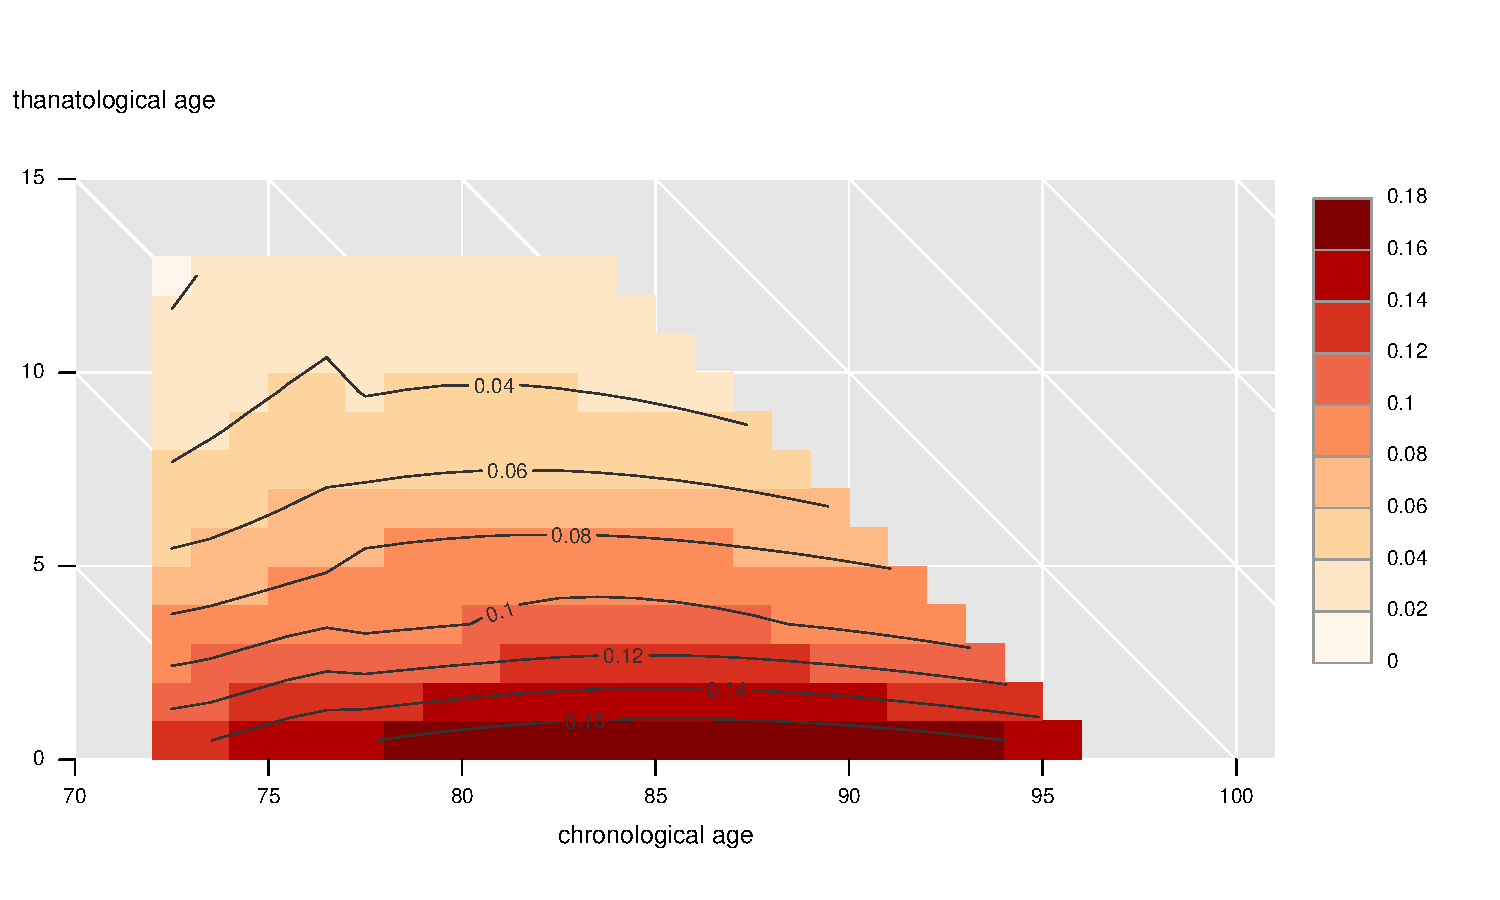
\includegraphics[scale=.6]{Figures/Figure2a.pdf}}
	\end{subfigure}
	
	\begin{subfigure}{\linewidth}
    \caption{Back Problems by
    years lived (x axis) and years left (y axis). Females, 1915-1919 birth
    cohort.}
    \label{fig:back}
	\vspace{-2em}
	\makebox[\textwidth][c]{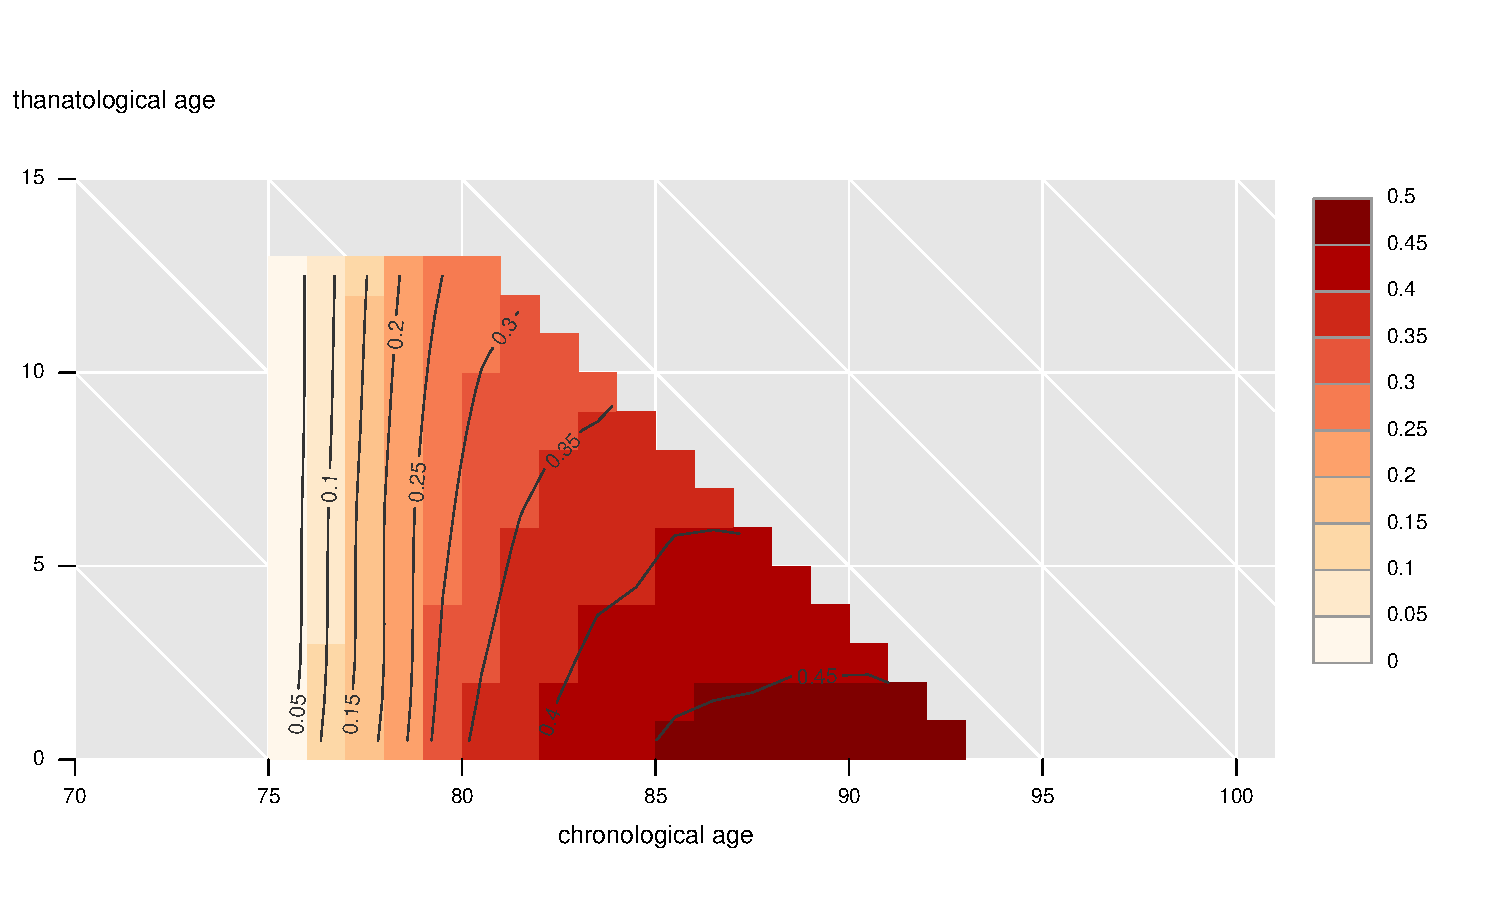
\includegraphics[scale=.6]{Figures/Figure2b.pdf}}
	\end{subfigure}
\end{figure}

\begin{figure}[!h]
 \centering
   \caption{Psychological problems (ever) by chronological age only. Males, 1915-1919 birth
    cohort. With 95{\%} confidence bands from loess fit.}
    \label{fig:chronofalse}
   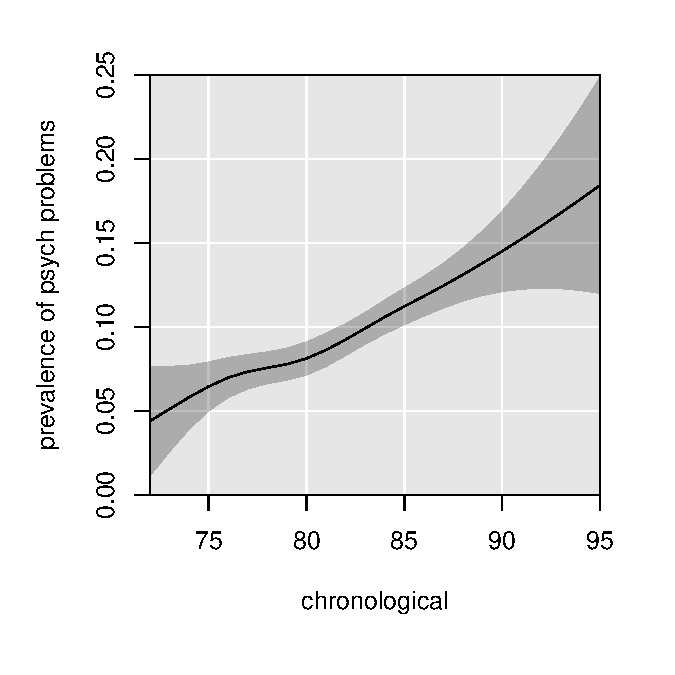
\includegraphics[scale=.7]{Figures/Figure3.pdf}
\end{figure}

Other informative patterns also exist among the set of characteristics studied.
These include characteristics that vary by lifespan, which display downward
diagonal contours in surface plots. Characteristics that vary by lifespan appear
constant within lifespans. These are often characteristics that \textit{determine} lifespan. Ever smoking displays such a pattern, as seen in
Figure~\ref{fig:evsmkng} for females of the 1915-1919 cohort. This pattern is
also a corroboration of science and common sense: smoking kills, eventually (at
least in this range of lifespans). Other variables that display similar patterns in this
window of the lifespan include lung disease among males (this is largely
redundant with the former), dental visits in the previous two years (females),
and diabetes among females. Sometimes such patterns combine in complex ways worthy of further study.

The fourth major pattern of contour variation runs perpendicular to lifelines.
One characteristic that clearly displays this pattern is ever having been
diagnosed with high blood pressure among males. This characteristic varies by
lifespan, and thanatological age within lifespan for this window of study.
In other words, longer lifespans display later onset but greater eventual odds of
having been diagnosed with high blood pressure. Arithmetically, $chronological~
age~-~thanatological~age$ is the operative predictor of blood pressure. For
example, for such characteristics, the condition of a 70-year old with five
remaining years of life may resemble that of an 80-year old with
15 remaining years of life. Such characteristics are not very useful alone for predicting eventual
lifespan.\footnote{We do not have expertise to comment further on blood
pressure, but instead only provide an interpretation of the surface presented.}
Some characteristics appear to follow this pattern, albeit with contour lines at
angles less than 45$^\circ$, which may suggest thanatological morbidity
prevalence somehow \textit{proportional} to length of life. We do not measure
this possibility explicitly.

\begin{figure}[!h]
    % This figure was produced in
    \centering
    \caption{Examples of characteristics that vary by lifespan only or by
    thanatological age within lifespan.}
    \label{fig:lifespan}
    \begin{subfigure}{\linewidth}
    \caption{Smoking (ever) by
    years lived (x axis) and years left (y axis). Females, 1915-1919 birth
    cohort.
    }
    \label{fig:evsmkng}
	\vspace{-2em}
	\makebox[\textwidth][c]{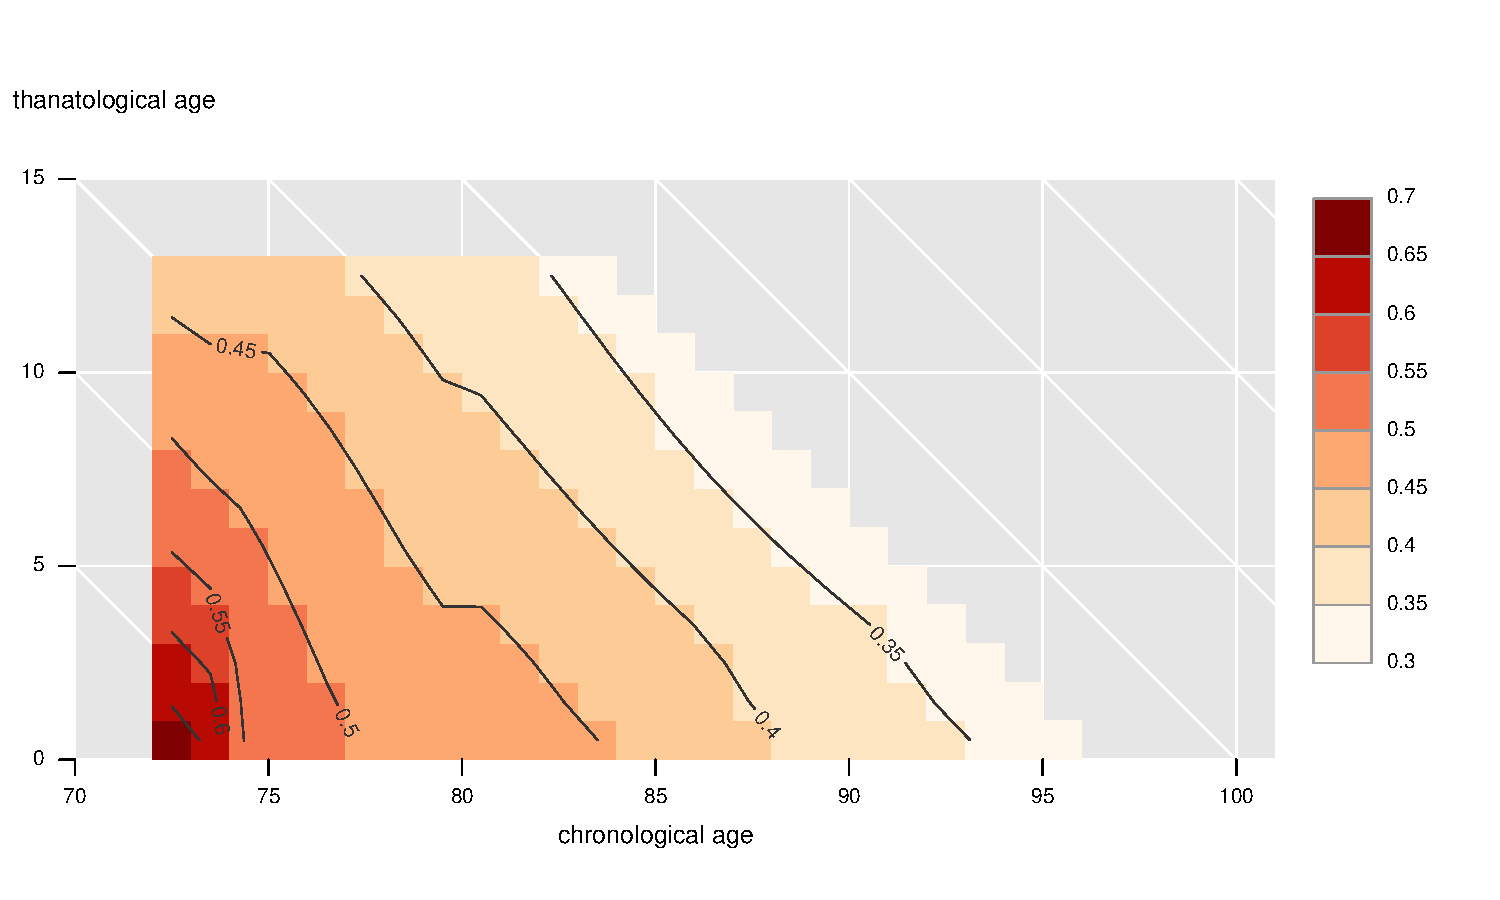
\includegraphics[scale=.6]{Figures/Figure4a.pdf}}
	\end{subfigure}
	
	\begin{subfigure}{\linewidth}
    \caption{Blood Pressure by
    years lived (x axis) and years left (y axis). Males, 1915-1919 birth
    cohort.}
    \label{fig:bp}
	\vspace{-2em}
	\makebox[\textwidth][c]{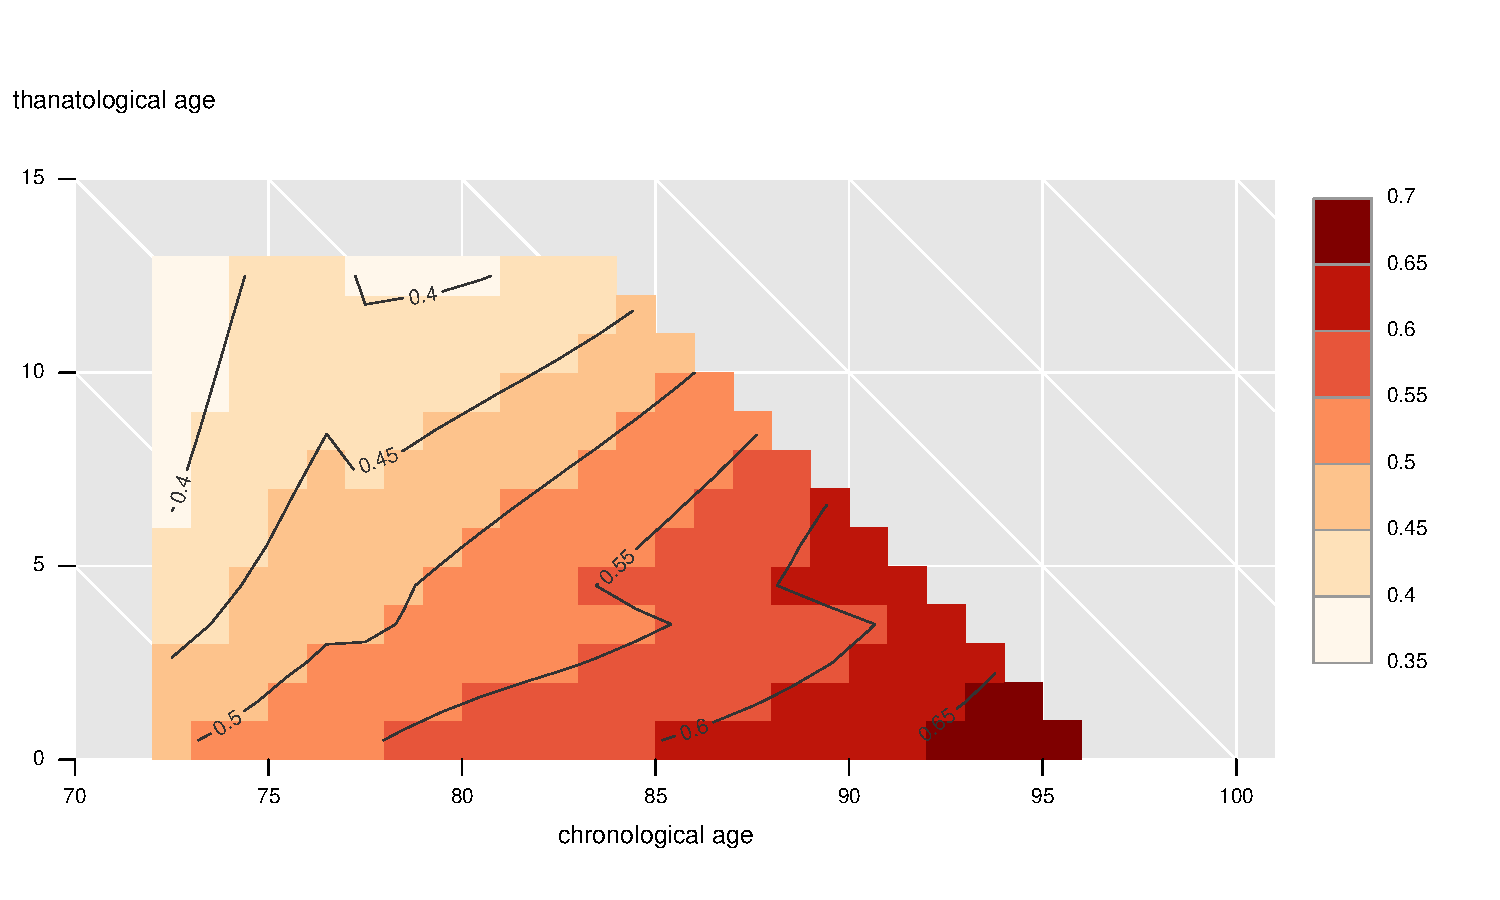
\includegraphics[scale=.6]{Figures/Figure4b.pdf}}
	\end{subfigure}
\end{figure}
\FloatBarrier



\paragraph{Summary of results for all characteristics}
We produce surfaces such as those in Figures~\ref{fig:thanochrono}
and~\ref{fig:lifespan} for all 78 variables and each sex. We distill each
of these surfaces into four Pearson correlation coefficients, each designed to
capture the variation along each of the four major patterns explained above. We
call the four patterns thanatological age (T), chronological age (A), lifespan
($A+T$) (L), and mixed ($A-T$) (M). Most characteristics are
well-summarized by either one or two of these patterns.
Figure~\ref{fig:correlations} shows the correlation coefficients of all 78
variables binned into count histograms for each sex and major variation pattern
separately. This view is meant to give a feel for how common each major
pattern of variation might be in commonly measured characteristics. This
statistic only captures the rough direction of variation in characteristics, and
it does not capture differences in levels or gradient steepness.

\begin{figure}
\centering
\caption{Distribution of correlation coefficients for each of the four major
patterns of variation, all 78 variables examined.
L indicates lifespan variation (like Figure~\ref{fig:evsmkng}), A chronological
age (like Figure~\ref{fig:back}), T thanatological age (like
Figure~\ref{fig:psych}), and M the mixed type variation (like
Figure~\ref{fig:bp}).}
\label{fig:correlations}
 \begin{subfigure}{.5\linewidth}
 \caption{Females}
  \vspace{-2em}
 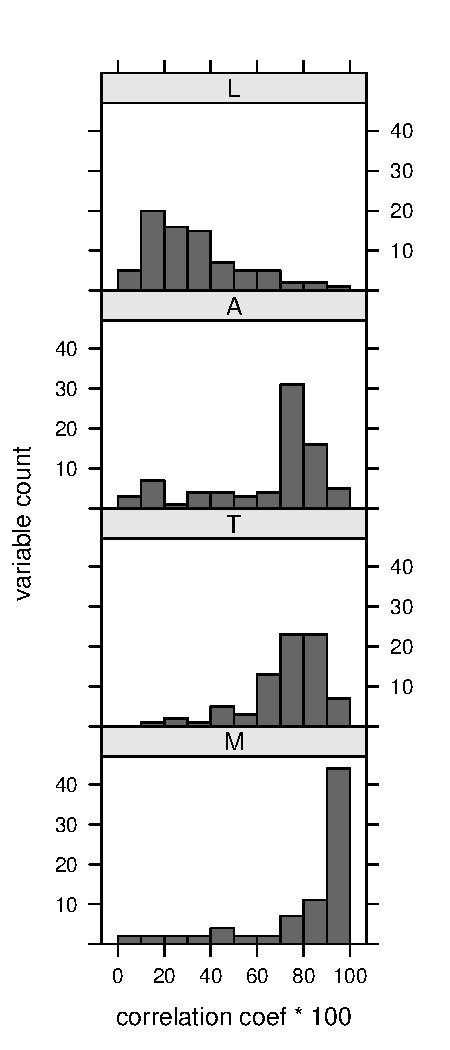
\includegraphics[scale=.8]{Figures/Figure5a.pdf}
 \end{subfigure}~
 \begin{subfigure}{.5\linewidth}
 \caption{Males}
 \vspace{-2em}
 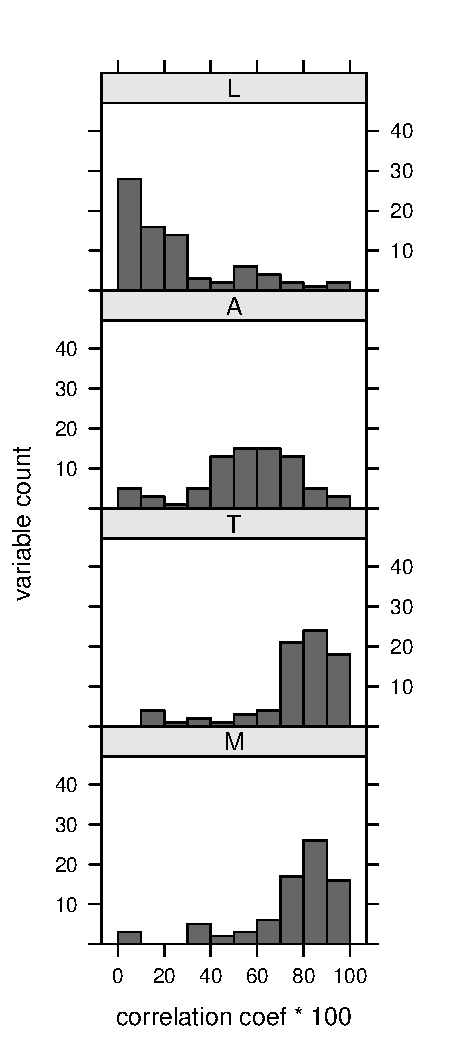
\includegraphics[scale=.8]{Figures/Figure5b.pdf}
 \end{subfigure}
\end{figure}

The first row of this panel shows that variation by lifespan is weak for most
variables, and strong for only a few (ever smoking, and for females having
visited a dentist).
The second row shows that chronological age is indeed an important aspect of variation for many characteristics, but not
all characteristics (e.g., ever having been diagnosed with pyschological
problems), and chronological variation is more often strong for females than for
males.
The third row shows that thanatological age is an important pattern of variation
for many variables: the lower tail is thinner than that of chronological age,
and there are more cases of strong correlations ($r>0.80$) in the direction of thanatological variation than
of chronological variation. In the distributions over these variables, males tend to
more commonly show stronger thanatological age patterns than females, and
females tend to show stronger chronological age patterns than males. Finally, the most common pattern in these data are for
characteristics to vary strongly as chronological age increases \textit{and} as
thanatological age decreases, M (especially for many ADLs, IADLs, functional
limitations, and many variables of cognitive funciton).
For females, this is very clearly the dominant pattern among the variables studied. For males, the pattern of variation between
characteristics is similar to that of thanatological age. In most cases, for
variables with strong patterns of variation in the M direction, there are also
strong correlations in the A and/or T directions. Of these, M is most commonly
paired with T. Characteristics that show strong correlation in both M and T
display surfaces with contour lines slanted less than $45^\circ$. A more
detailed table of correlation results by variable, pattern, and sex is given in
the appendix.

\FloatBarrier
\section*{Discussion}
The distribution of tested characteristics with respect to the
four primary patterns of variation is
striking. Chronological age describes prevalence patterns for many conditions
well, but time-to-death patterns are more prevalent among the measures
tested.
For measures that vary both with the increase of age and the approach to death, the approach to
death is more often the stronger of the two measures. Characteristics that vary
by length of life are few, but their patterns are clear. The upshot, as
illustrated by comparing figures \ref{fig:psych} and \ref{fig:chronofalse}, is
that representing morbidity or disability variables as chronological age
patterns can in many or most cases be misleading as model of morbidity
processes, and biased as a basis for prediction.

These empirical
findings must be tempered by noting that 1) the summary measure (correlation
coefficient) used here blends out some information, 2) these results may not
extrapolate to the set of all testable questions in the HRS, and 3)
this relationship does not necessarily hold in other windows of the lifespan or
other birth cohorts. Comparable results for other five-year birth cohorts
in the HRS (1905-1925) are given in the manuscript repository. 

Further, the patterns
presented here are valid for the whole population (of a given sex) taken
together, but were the target population broken down by causes of death (for
instance), the patterns may change. For example, imagine hypothetically that the
strong thanatological pattern shown in Figure~\ref{fig:thanochrono}
(psychological problems) were driven by strong patterns within individuals that
eventually die of suicide, but that other causes of death displayed entirely different patterns with respect to
psychological problems. Such cases are easily imaginable for other
characteristics and causes of death. At the time of this research, we did not
have access to cause of death information from the HRS mortality followup. For
detailed investigations of particular characteristics, cause-conditioning
surfaces would clearly aid in disentangling morbidity processes, both for
purposes of understanding and for cause and time of death prediction.

Research to better document the multidimensional age variation of particular
characteristics would benefit from more empirical evidence and further model
development.
Despite the limitation of this study, we have been able to demonstrate the
complex variety of age and lifespan dimensions over which some key aspects of the aging process unfold. All of the indicators we tested are commonly used to describe population aging, and
very few of them are exclusively a function of chronological age. If this
finding is sustained in other cohorts and populations, and if other indicators
here untested also display similar temporal complexity, we submit that the
common discourse and debate on the nature and impacts of aging ought to be
better informed by more judicious measurement and description in terms of
thanatological as well as chronological age. This would benefit scientific
understanding of health and disability processes, and it would improve
the actuarial accuracy of morbidity projections and any policies that count
on accurate morbidity projections. 

That accounting for time-to-death in predictions of
healthcare expenditure reduces bias has already been established in the health
economics literature \citep[e.g.,][]{stearns2004time}. A common finding
on healthcare expenditure prediction is that in times of mortality improvements,
predictions based on chronological age patterns of healthcare
expenditure (Sullivan-style predictions \citep{sullivan1970}) tend
to overestimate total expenditure \citep[e.g.,][]{geue2014population}. 
Since the patterns of variation among the morbidity dimensions we study are
similar to those of healthcare expenditure over chronological age and
time-to-death, we here infer that Sullivan-style predictions of morbidity are
biased in the same direction.\footnote{Other work in progress treats this point
in greater detail \citep{vanRaalte2015HLE}.} The consequences of overestimating
future morbidity prevalence are complex and varied, ranging from
budget misallocations, poor design of social healthcare systems for the elderly,
through to to lowered expectations on the benefits of lengthening life.

We hope that the conceptual model of the
lifecourse presented here, which complements the Lexis diagram, will be of use
to demographers, public health researchers, and epidemiologists. Other combinations
of lifespan time dimensions are also possible, and these would highlight
different patterns in data \citep{rsv2015}. The variety and availability of such
options, perhaps now placed in starker relief, demands a more nuanced understanding of the temporal accounting that relates demographic time
perspectives. Further exploration and experimentation with these formal
demographic concepts will lead to a more precise toolkit for demographic
measurement and the practice of demography, and ultimately a wiser contribution
to the discourse on population aging.

We suggest a selection of extensions to the exploration carried out here. The
present variety of analysis must be replicated for more cohorts and populations. A few populations with long-running and fully linked population registers already preside over such information, and we encourage a
more thorough exploration of the temporal richness in population change and
population characteristics. 
Large scale panel studies may be motivated to implement, increase, or improve the quality of mortality follow-up modules. Information on the full age dimensions of health
outcomes will be valuable. The good news is that many unlinked panel studies may be linked to death registers in retrospect. 

If compared over calendar time, demographic work such as this will
provide a more precise answer to the question of morbidity compression. Given the chronological-age ruse exemplified in the case of psychological problems (see Figures~\ref{fig:chronofalse} versus~\ref{fig:psych}), it is safe to say that unless retrospective
thanatological measurements of morbidity dimensions are undertaken, we do
not have direct information about whether compression is (or has
been) happening or not. Using the techniques shown here, the researcher may
directly estimate the varieties of end-of-life profiles often seen in the
literature on morbidity compression \citep[e.g.,][]{fries2011compression}.

There are also consequences for the popular understanding of aging. By
using analyses oriented by the lifecourse diagram, health care providers better situate the association of certain health outcomes with stages of the aging process. This is both a question of allocating resources and a question of how individuals conceive of
themselves with respect to age. In this regard, we add to the chorus of
researchers working to change the measurement of age to reflect the changing
experience of age \citep[see e.g.,][]{sanderson2013characteristics}. 

The lifecourse surfaces underlying this study highlight important sex
differences in the aggregate onset and trajectory of some aspects of morbidity.
Some of these differences may corroborate extant findings, such as the
male-female health-survival paradox, and others may provide new understanding to
sexual dimorphism in morbidity. Specifically, females have been found to live
longer but in worse health than males \citep[e.g.,][]{case2005sex}, and this is
consistent with females having somewhat more chronologically-varying health
patterns than males. In general, these methods and measurements are
applicable to describe any between-group disparity in demographic or social outcomes, especially those that directly or indirectly relate to remaining years of life. Numerous other avenues of potential investigation may also be devised from the present work. It is our hope that these results are strongly suggestive and orient future investigation.

%\FloatBarrier
\singlespacing
\bibliographystyle{chicago}
  \bibliography{references} 
%  

%\pagebreak

\begin{appendices}
\section*{Appendix: Variables and correlations}

For tables displayed in this appendix we use a shorthand to identify axis types.
\texttt{T} indicates the correlation coefficient along the thanatological age axis.
\texttt{A} indicates the chronological age axis. \texttt{L} indicates the lifespan axis
(right-downward slanting isolines), the least common in these data. \texttt{M}
indicates the mixed axis, upward-right slanting isolines, the most common type
in these data.
The code used to generate these and all other results, including results for all 5-year cohorts from 1905-1925 and different
degrees of smoothing, is available freely the repository. The repository
also contains a csv of these summary results.

\url{https://github.com/timriffe/ThanoEmpirical}

Results are grouped by several major morbidity categories and presented in
heatmap tables. In these tables, darker shades of grey indicate higher
correlations (black = 1), and lighter grays indicate low correlations
(white = 0). Numbers inside the cells indicate the rounded Pearson's correlation
coefficient $\times$ 100, and can be interpreted as percents. 

Finally, it bears noting that these values say nothing of prevalence levels.
They are only intended to be rough gauges of the direction of variation in characteristics.

\listoftables

\pagebreak
%-------------------------------------
% ADL
\begin{table}
\centering
\caption{Activities of Daily Living (ADL)}
\label{tab:adl}
\begin{tabular}{L{2.5cm}|L{3cm}C{3.2cm}C{3.2cm}}
Short & Description & Females & Males \\
      &      & \texttt{L~~~A~~~T~~~M} &  \texttt{L~~~A~~~T~~~M} \\ \toprule
ADL3 & ADL 3 point & \hm{f}{adl3} & \hm{m}{adl3} \\
ADL5 & ADL 5 point & \hm{f}{adl5} & \hm{m}{adl5} \\
WALK & Difficulty walking across room & \hm{f}{adlwalk} & \hm{m}{adlwalk} \\
DRESS & Difficulty dressing & \hm{f}{adldress} & \hm{m}{adldress} \\
BATH & Difficulty bathing or showering  & \hm{f}{adlbath} &\hm{m}{adlbath} \\
EAT & Difficuty eating  & \hm{f}{adleat} &\hm{m}{adleat} \\
BED & Difficuty getting in/out bed  & \hm{f}{adlbed} &\hm{m}{adlbed} \\
TOILET & Difficulty using toilet & \hm{f}{adltoilet} &\hm{m}{adltoilet} \\
\bottomrule
\end{tabular}
\end{table}

%-------------------------------------
% IADL
\begin{table}
\centering
\caption{Instrumental Activities of Daily Living (IADL)}
\label{tab:iadl}
\begin{tabular}{L{2.5cm}|L{3cm}C{3.2cm}C{3.2cm}}
Short & Description & Females & Males \\
      &      & \texttt{L~~~A~~~T~~~M} &  \texttt{L~~~A~~~T~~~M} \\ \toprule
IADL3 & IADL 3 point & \hm{f}{iadl3} & \hm{m}{iadl3} \\
IADL5 & IADL 5 point & \hm{f}{iadl5} & \hm{m}{iadl5} \\
WORK & Health limits work & \hm{f}{limwork} & \hm{m}{limwork} \\
MAP & Difficulty using maps & \hm{f}{iadlmap} & \hm{m}{iadlmap} \\
TEL & Difficulty using telephone & \hm{f}{iadltel} & \hm{m}{iadltel} \\
MONEY & Difficulty managing money & \hm{f}{iadlmoney} & \hm{m}{iadlmoney} \\
MEDS & Difficulty taking medications & \hm{f}{iadlmeds} & \hm{m}{iadlmeds} \\
SHOP & Difficulty grocery shopping &  \hm{f}{iadlshop} &
\hm{m}{iadlshop}\\
MEALS & Difficulty prep. hot meals &  \hm{f}{iadlmeals} & \hm{m}{iadlmeals} \\
\bottomrule
\end{tabular}
\end{table}

%-------------------------------------
% Health behaviors
\begin{table}
\centering
\caption{Health behaviors}
\label{tab:health}
\begin{tabular}{L{2.5cm}|L{3cm}C{3.2cm}C{3.2cm}}
Short & Description & Females & Males \\
      &      & \texttt{L~~~A~~~T~~~M} &  \texttt{L~~~A~~~T~~~M} \\ \toprule
ALCEV & Alcohol, ever-drinker  & \hm{f}{alcev} & \hm{m}{alcev} \\
ALCDAYS & Drinking days / week  & \hm{f}{alcdays} & \hm{m}{alcdays} \\
ALCDRINKS & Nr drinks per drinking day  & \hm{f}{alcdrinks} & \hm{m}{alcdrinks} \\
SMOKEEV & Ever-smoker & \hm{f}{smokeev} & \hm{m}{smokeev} \\
SMOKECUR & Current-smoker & \hm{f}{smokecur} & \hm{m}{smokecur} \\
\bottomrule
\end{tabular}
\end{table}

%-------------------------------------
% Functional limitations
\begin{table}
\centering
\caption{Functional limitations}
\label{tab:func}
\begin{tabular}{L{2.5cm}|L{3cm}C{3.2cm}C{3.2cm}}
Short & Description & Females & Males \\
      &      & \texttt{L~~~A~~~T~~~M} &  \texttt{L~~~A~~~T~~~M} \\ \toprule
BMI & Body mass index  & \hm{f}{bmi} & \hm{m}{bmi} \\
BACK & Back problems  & \hm{f}{back} & \hm{m}{back} \\
MOB & Mobility difficulty index & \hm{f}{mob} & \hm{m}{mob} \\
LGMUS & Large muscle difficulty index & \hm{f}{lgmus} & \hm{m}{lgmus} \\
GROSSMOT & Gross motor difficulty index & \hm{f}{grossmot} & \hm{m}{grossmot}\\
FINEMOT & Fine motor difficulty index & \hm{f}{finemot} & \hm{m}{finemot}\\
\bottomrule
\end{tabular}
\end{table}

%-------------------------------------
%  Chronic conditions
\begin{table}
\centering
\caption{Chronic conditions}
\label{tab:chron}
\begin{tabular}{L{2.5cm}|L{3cm}C{3.2cm}C{3.2cm}}
Short & Description & Females & Males \\
      &      & \texttt{L~~~A~~~T~~~M} &  \texttt{L~~~A~~~T~~~M} \\ \toprule
CC & Number of chronic conditions & \hm{f}{cc} & \hm{m}{cc} \\
BP & High blood pressure, ever & \hm{f}{bp} & \hm{m}{bp} \\
DIAB & Diabetes, ever & \hm{f}{diab} & \hm{m}{diab} \\
CANCER & Cancer, ever & \hm{f}{cancer} & \hm{m}{cancer} \\
LUNG & Lung disease & \hm{f}{lung} & \hm{m}{lung} \\
HEART & Heart problems, ever  & \hm{f}{heart} & \hm{m}{heart} \\
STROKE & Stroke, ever  & \hm{f}{stroke} & \hm{m}{stroke} \\
PSYCH & Psychological problems , ever  & \hm{f}{psych} & \hm{m}{psych} \\
ARTH & Arthritis, ever  & \hm{f}{arth} & \hm{m}{arth} \\
\bottomrule
\end{tabular}
\end{table}

%-------------------------------------
%  Cognitive function
\begin{table}
\centering
\caption{Cognitive function}
\label{tab:cog}
\begin{tabular}{L{2.5cm}|L{3cm}C{3.2cm}C{3.2cm}}
Short & Description & Females & Males \\
      &      & \texttt{L~~~A~~~T~~~M} &  \texttt{L~~~A~~~T~~~M} \\ \toprule
SRM & Self-rated memory & \hm{f}{srm} & \hm{m}{srm} \\
PASTMEM & Memory compared to past & \hm{f}{pastmem} & \hm{m}{pastmem} \\
SS & Serial 7s & \hm{f}{ss} & \hm{m}{ss}\\
C20B & Backwards counting &  \hm{f}{c20b} & \hm{m}{c20b}\\
NAMEMO & Naming month &  \hm{f}{namemo} & \hm{m}{namemo}\\
NAMEDMO & Naming day of month &  \hm{f}{namedmo} & \hm{m}{namedmo}\\
NAMEYR & Naming year &  \hm{f}{nameyr} & \hm{m}{nameyr}\\
NAMEDWK & Naming day of week &  \hm{f}{namedwk} & \hm{m}{namedwk}\\
NAMESCI & Naming scissors &  \hm{f}{namesci} & \hm{m}{namesci}\\
NAMECAC & Naming cactus &  \hm{f}{namecac} & \hm{m}{namecac}\\
NAMEPRES & Naming president &  \hm{f}{namepres} & \hm{m}{namepres}\\
NAMEVP & Naming vice president &  \hm{f}{namevp} & \hm{m}{namevp}\\
VOCAB & Vocabulary score & \hm{f}{vocab} & \hm{m}{vocab}\\
TM & Mental status summary & \hm{f}{tm} & \hm{m}{tm}\\
DWR & Delayed word recall & \hm{f}{dwr} & \hm{m}{dwr}\\
TWR & Total word recall & \hm{f}{twr} & \hm{m}{twr}\\
IWR & Delayed word recall & \hm{f}{iwr} & \hm{m}{iwr}\\
\bottomrule
\end{tabular}
\end{table}

% -------------------------
% Psychological wellbeing
\begin{table}
\centering
\caption{Psychological wellbeing}
\label{tab:psych}
\begin{tabular}{L{2.5cm}|L{3cm}C{3.2cm}C{3.2cm}}
Short & Description & Females & Males \\
      &      & \texttt{L~~~A~~~T~~~M} &  \texttt{L~~~A~~~T~~~M} \\ \toprule
CESD & Depression score & \hm{f}{cesd} & \hm{m}{cesd} \\
SRH & Self-reported health & \hm{f}{srh} & \hm{m}{srh} \\
DEPR & Felt depressed & \hm{f}{cesddepr} & \hm{m}{cesddepr} \\
SLEEP & Sleep restless  & \hm{f}{cesdsleep} & \hm{m}{cesdsleep} \\
HAPPY & Was happy  & \hm{f}{cesdhappy} & \hm{m}{cesdhappy} \\
LONE & Felt lonely  & \hm{f}{cesdlone} & \hm{m}{cesdlone} \\
SAD & Felt sad  & \hm{f}{cesdsad} & \hm{m}{cesdsad} \\
GOING & Could not get going & \hm{f}{cesdgoing} & \hm{m}{cesdgoing} \\
ENJOY & Enjoyed life & \hm{f}{cesdenjoy} & \hm{m}{cesdenjoy} \\
\bottomrule
\end{tabular}
\end{table}

% -------------------------
% healthcare use
\begin{table}
\centering
\caption{Healthcare use (24 months)}
\label{tab:hu}
\begin{tabular}{L{2.5cm}|L{3cm}C{3.2cm}C{3.2cm}}
Short & Description & Females & Males \\
      &      & \texttt{L~~~A~~~T~~~M} &  \texttt{L~~~A~~~T~~~M} \\ \toprule
HOSP & Overnight hospital & \hm{f}{hosp} & \hm{m}{hosp} \\
HOSPSTAYS & Number hospital stays & \hm{f}{hospstays} & \hm{m}{hospstays} \\
HOSPNIGHTS & Number nights in hospitals & \hm{f}{hospnights} &\hm{m}{hospnights} \\
NH & Overnight stay in nursing home & \hm{f}{nh} &\hm{m}{nh} \\
NHSTAYS & Nursing home stays & \hm{f}{nhstays} &\hm{m}{nhstays} \\
NHNIGHTS & Number nights in nursing homes & \hm{f}{nhnights} &\hm{m}{nhnights} \\
NHNOW & Nursing home at interview & \hm{f}{nhnow} &\hm{m}{nhnow} \\
DOC & Visited doctor & \hm{f}{doc} &\hm{m}{doc} \\
DOCVISITS & Number of doctor visits & \hm{f}{docvisits} &\hm{m}{docvisits} \\
HHC & Home health care & \hm{f}{hhc} &\hm{m}{hhc} \\
MEDS & Prescription drugs regularly & \hm{f}{meds} &\hm{m}{meds} \\
SURG & Outpatient surgery & \hm{f}{surg} &\hm{m}{surg} \\
DENT & Visited dentist & \hm{f}{dent} &\hm{m}{dent} \\
SHF & Visited special healthcare facility & \hm{f}{shf} &\hm{m}{shf} \\
\bottomrule
\end{tabular}
\end{table}

  \end{appendices}
\end{document}